\documentclass{beamer}
\usetheme{Boadilla}
\usepackage{bibentry}
%\usepackage{cmbright}
\usepackage{natbib}
\setbeamertemplate{itemize items}[circle]
\setbeamertemplate{enumerate items}[default]

\def\E{\mathbb{E}}
\def\Var{\mathrm{Var}}

\title[Implied Rates]{\textbf{Limited Asset Market Participation} and the Euler Equation Implied Rate}
\author{Pearl Li}
\date{April 6, 2016}

\begin{document}



\begin{frame}
\titlepage
\end{frame}

\begin{frame}{Previously: Aggregate Analysis}
\begin{itemize}
\item Data from NIPA
\item Estimated VAR(4) for consumption, inflation, leisure, FFR, ...
\item Computed implied interest rates with and without
  \begin{enumerate}
  \item Habit formation
  \item Nonseparability in consumption and leisure
  \end{enumerate}
\item Regressed (implied - observed) spread against stance of monetary policy
\item Computed impulse response functions for implied rates
\end{itemize}
\end{frame}

\begin{frame}{Limited Asset Market Participation}
\begin{itemize}
\item Inspired by
  \begin{itemize}
  \item \cite{campbell89}: estimated half of aggregate consumption undertaken by households who don't optimize
  \item \cite{vissing02}: estimated EIS separately for stock-, bond-, and non-assetholders
  \end{itemize}
\item Aggregate household-level data for bondholders and nonbondholders
\item Repeat analysis from before, comparing bondholders and nonbondholders
\item \textbf{Hypothesis: interest rates implied by bondholders' consumption paths will more resemble observed rates than those from nonbondholders}
\end{itemize}
\end{frame}

\begin{frame}{Data}
\begin{itemize}
\item Consumer Expenditure Survey, 1996.I to 2012.IV
\item Rotating panel of representative households, interviewed for 5 quarters (1 practice)
\item Very detailed household-level expenditure categories
\item Demographic and income data collected in 2nd and 5th interviews
\end{itemize}
\end{frame}

\begin{frame}{Bondholder Criteria}
\begin{itemize}
\item Following \cite{vissing02}
\item Asset holdings information only collected in 5th interview
\item Positive response to at least one of:
  \begin{enumerate}
  \item Stock, bonds, and mutual funds category
  \item U.S. savings bond category
  \end{enumerate}
\item Household classified as bondholder if at least one of:
  \begin{enumerate}
  \item Same amount of asset as a year ago and positive amount in interview
  \item Lower holdings of asset than a year ago
  \item Increase in holdings by less than reported holdings in interview
  \end{enumerate}
\end{itemize}
\end{frame}

\begin{frame}{More Specifications}
\begin{itemize}
\item Following \cite{heathcote10}:
  \begin{itemize}
  \item Nondurable consumption := food, clothing, gasoline, household operation, transportation, medical care, recreation, tobacco, and education
  \end{itemize}
\item Following \cite{krueger15}:
  \begin{itemize}
  \item Disposable income := after-tax income
  \end{itemize}
\item Following \cite{vissing02}:
  \begin{itemize}
  \item Consumption and income deflated using CPI-U nondurables (2009 dollars)
  \end{itemize}
\end{itemize}
\end{frame}

\begin{frame}{More Specifications}
\begin{itemize}
\item Output less consumption := before-tax income - consumption
\item Aggregated using CEX-provided population weights
\item Inflation, FFR, and CCI series from aggregate analysis
\item Log of real consumption seasonally-adjusted by hand
\end{itemize}
\end{frame}

\begin{frame}{Household-Level Summary Stats}
\begin{center}
\begin{tabular}{lcccc}
                  & \multicolumn{2}{c}{Bondholders} & \multicolumn{2}{c}{Nonbondholders} \\
                  & Mean   & SD                     & Mean   & SD \\ \hline
Consumption       & 1,774  & 1,886                  & 1,245  & 1,339 \\
After-Tax Income  & 70,641 & 64,604                 & 48,288 & 50,043 \\
Hours Worked/Week & 41.1   & 13.1                   & 40.5   & 12.3 \\ \hline
Observations      & \multicolumn{2}{c}{167,541}     & \multicolumn{2}{c}{1,009,032} \\
Households        & \multicolumn{2}{c}{16,959}      & \multicolumn{2}{c}{125,895} \\ \hline
\end{tabular} \\
(All dollar amounts nominal)
\end{center}
\end{frame}

\begin{frame}{Volatility Problem}
\begin{center}
\begin{tabular}{ccc}
NIPA & CEX Bond & CEX Nonbond \\
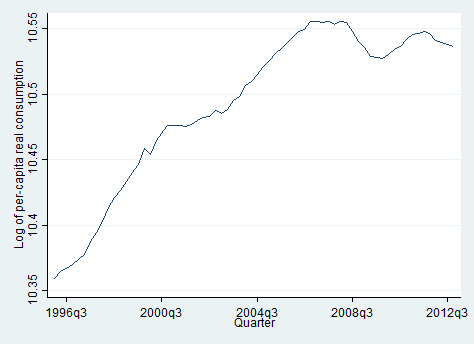
\includegraphics[width=0.3\textwidth]{figs/series/nipa_log-consumption} & 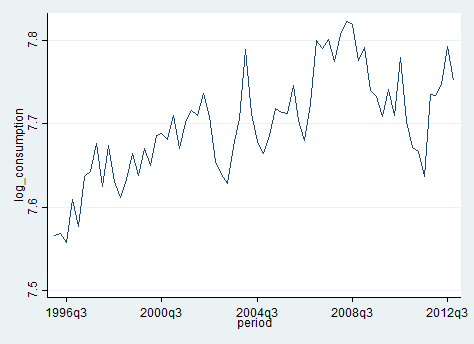
\includegraphics[width=0.3\textwidth]{figs/series/cex-bondholders_log-consumption} & 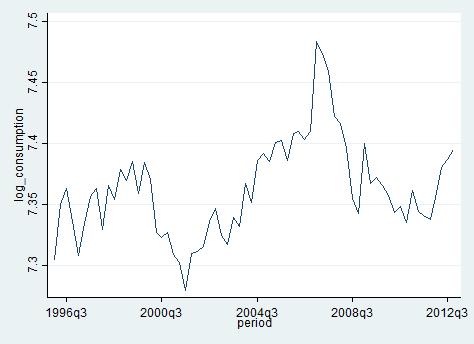
\includegraphics[width=0.3\textwidth]{figs/series/cex-nonbondholders_log-consumption} \\
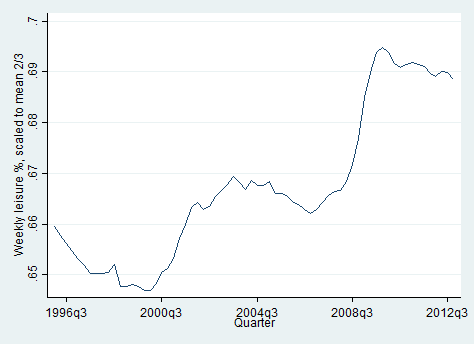
\includegraphics[width=0.3\textwidth]{figs/series/nipa_scaled-leisure-pct} & 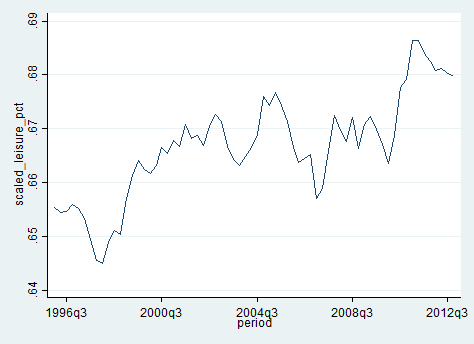
\includegraphics[width=0.3\textwidth]{figs/series/cex-bondholders_scaled-leisure-pct} & 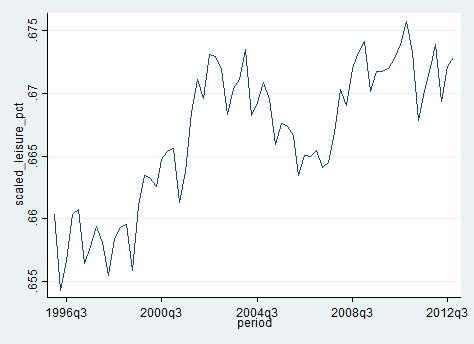
\includegraphics[width=0.3\textwidth]{figs/series/cex-nonbondholders_scaled-leisure-pct}
\end{tabular} \\
Need much lower risk aversion to accommodate these consumption fluctuations...
\end{center}
\end{frame}

\begin{frame}{CRRA Implied Rates}
\begin{itemize}
\item Implied rates computed only from CRRA utility (no habit formation or nonseparability) $$u(C_t) = \frac{C_t^{1-\alpha}}{1-\alpha}$$
\item Euler equation $$\frac{1}{1+r_t} = \beta \frac{\E_t u'(C_{t+1})}{u'(C_t)} = \beta \left( \frac{\E_t C_{t+1}}{C_t} \right)^{-\alpha}$$
\item Coefficient of relative risk aversion $\alpha$
\end{itemize}
\end{frame}

\begin{frame}{Results: Nominal}
\begin{center}
\begin{tabular}{cc}
Bondholders & Nonbondholders \\
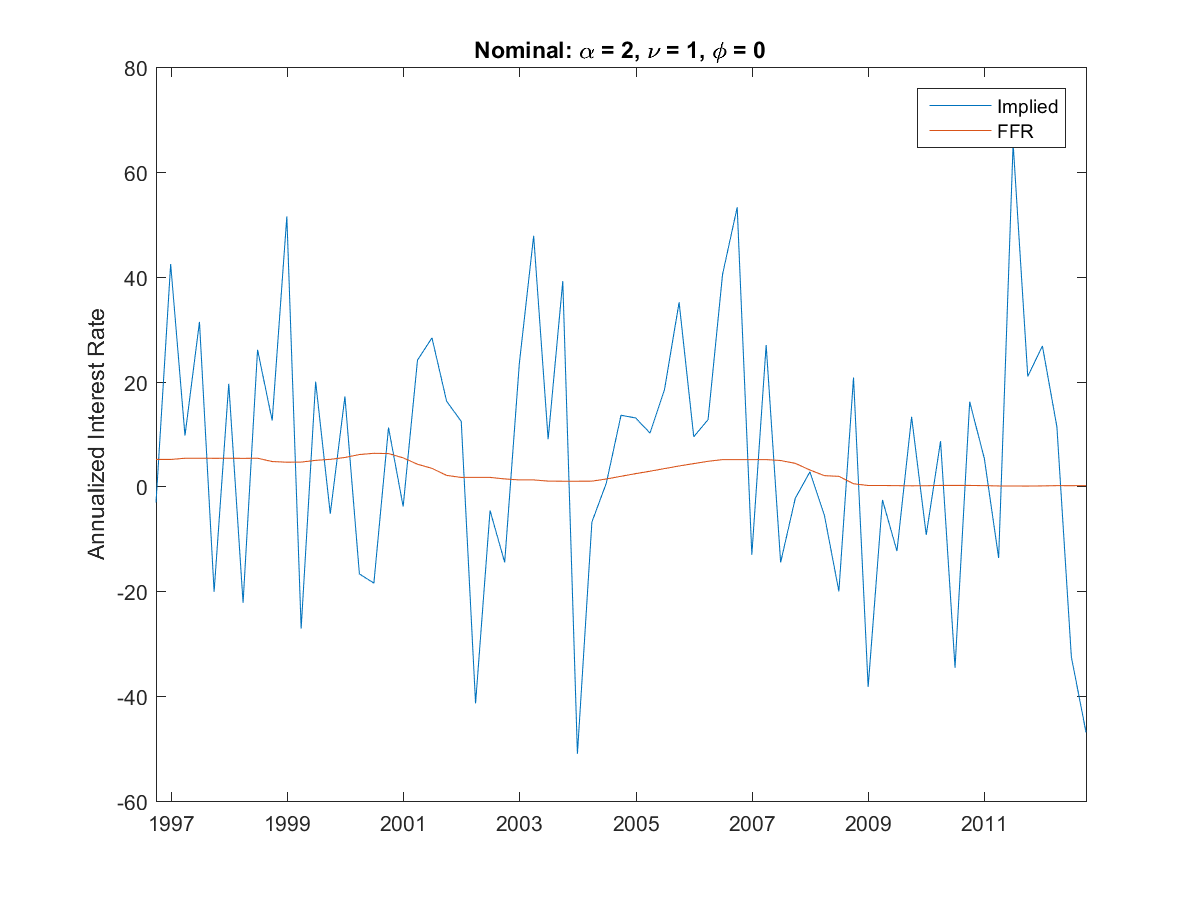
\includegraphics[width=0.4\textwidth]{figs/implied-vs-ffr/cex-bondholders/nominal_alpha2} & 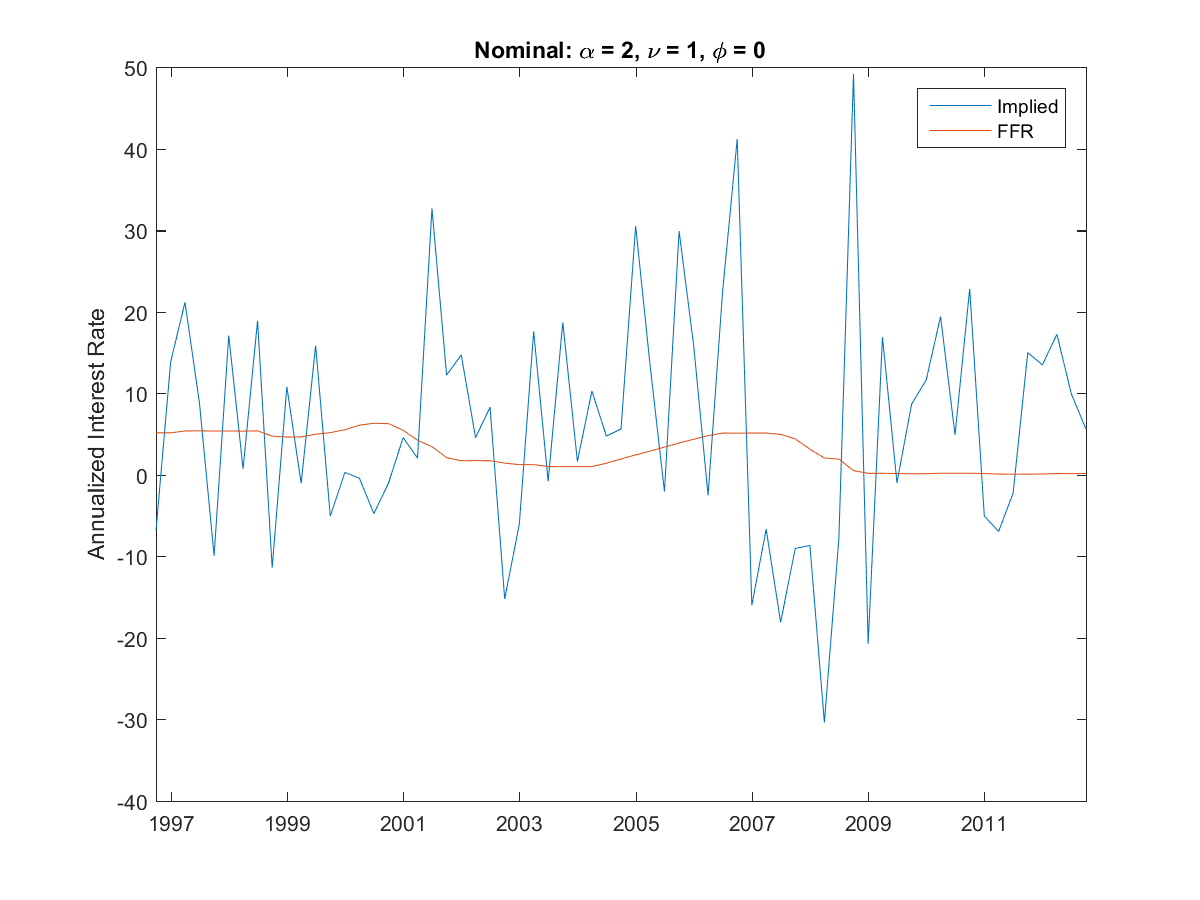
\includegraphics[width=0.4\textwidth]{figs/implied-vs-ffr/cex-nonbondholders/nominal_alpha2} \\
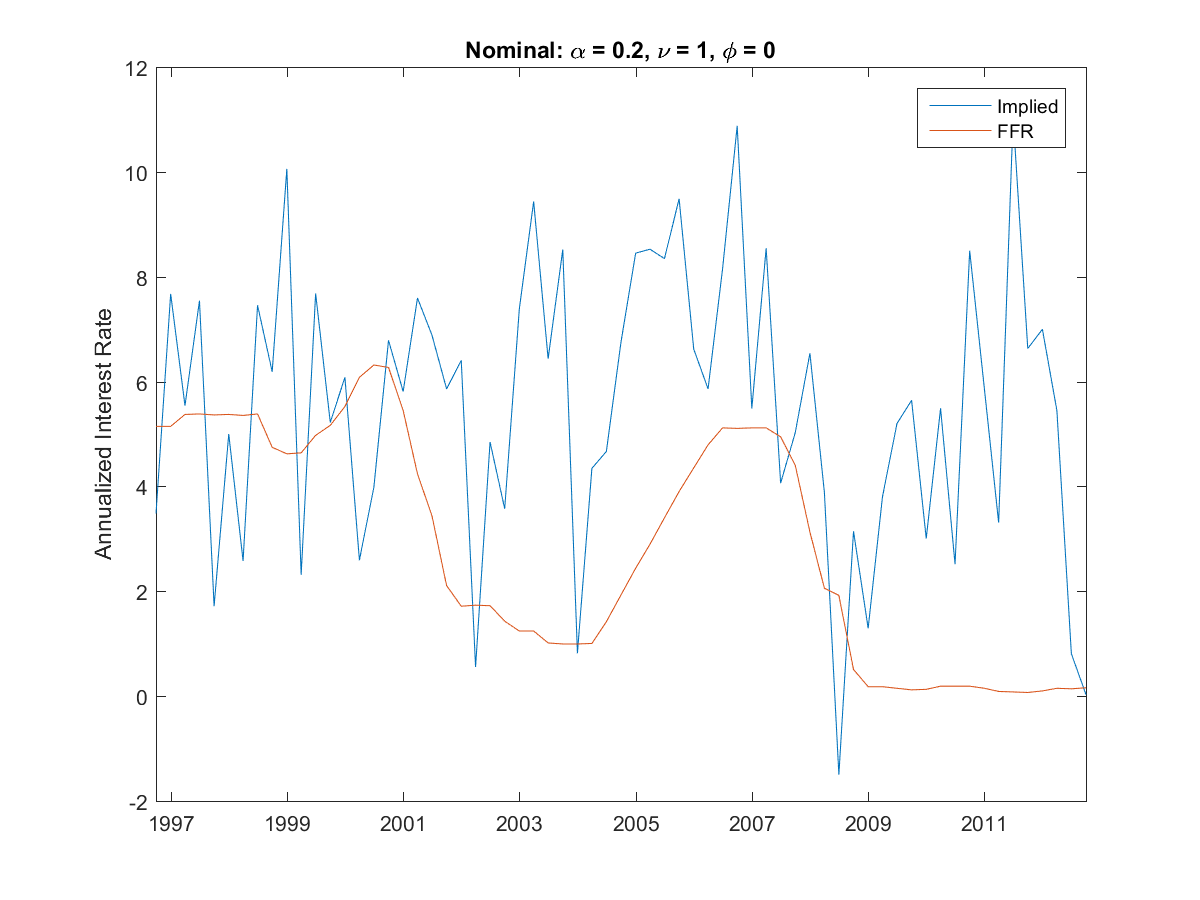
\includegraphics[width=0.4\textwidth]{figs/implied-vs-ffr/cex-bondholders/nominal_alpha_point2} & 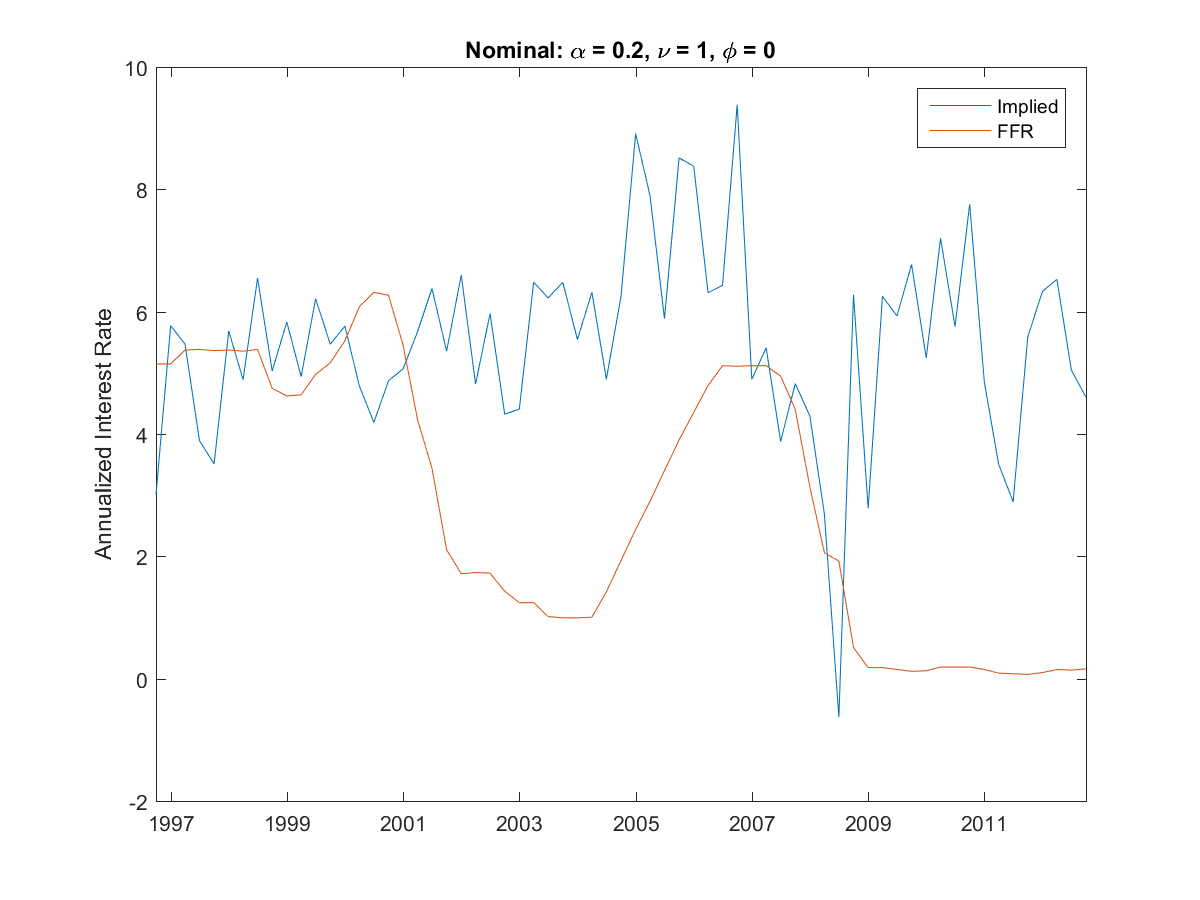
\includegraphics[width=0.4\textwidth]{figs/implied-vs-ffr/cex-nonbondholders/nominal_alpha_point2}
\end{tabular}
\end{center}
\end{frame}

\begin{frame}{Results: Real}
\begin{center}
\begin{tabular}{cc}
Bondholders & Nonbondholders \\
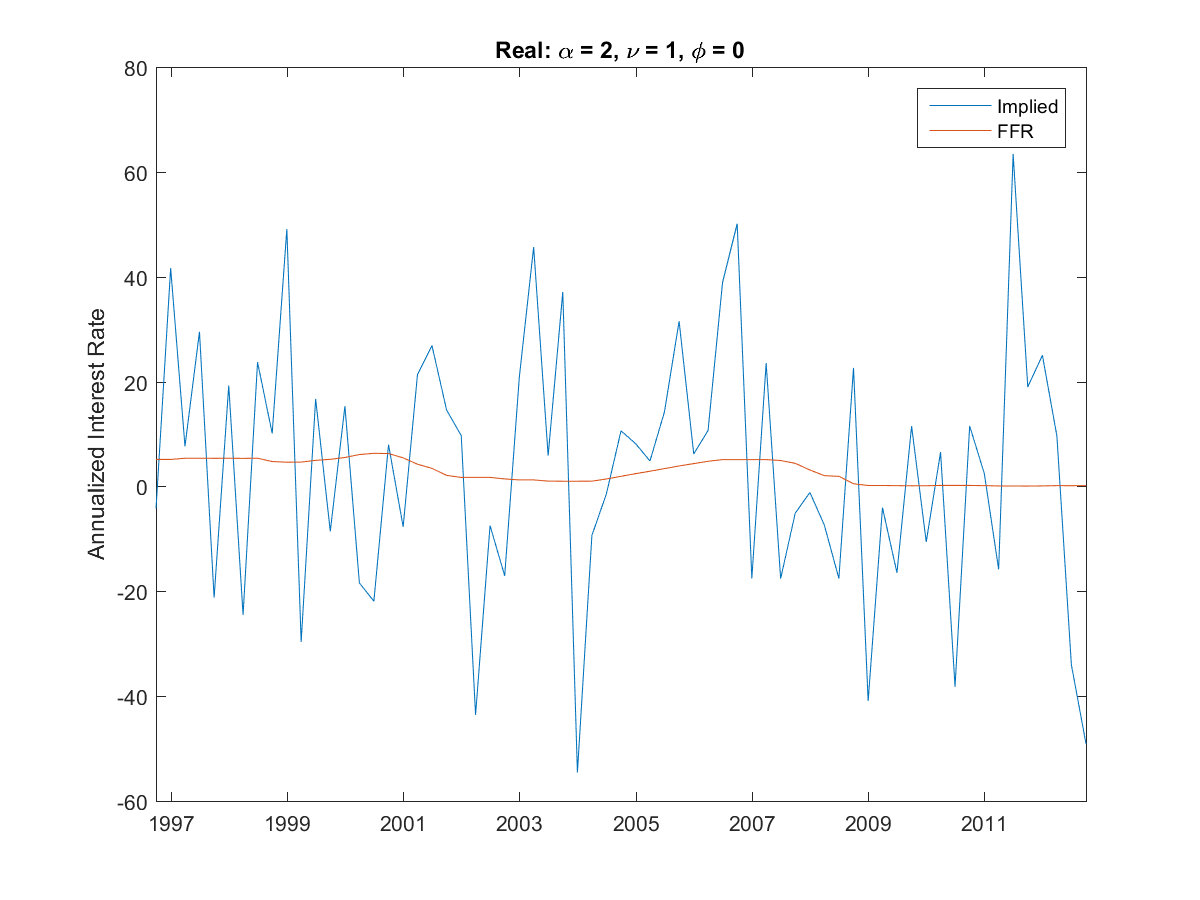
\includegraphics[width=0.4\textwidth]{figs/implied-vs-ffr/cex-bondholders/real_alpha2} & 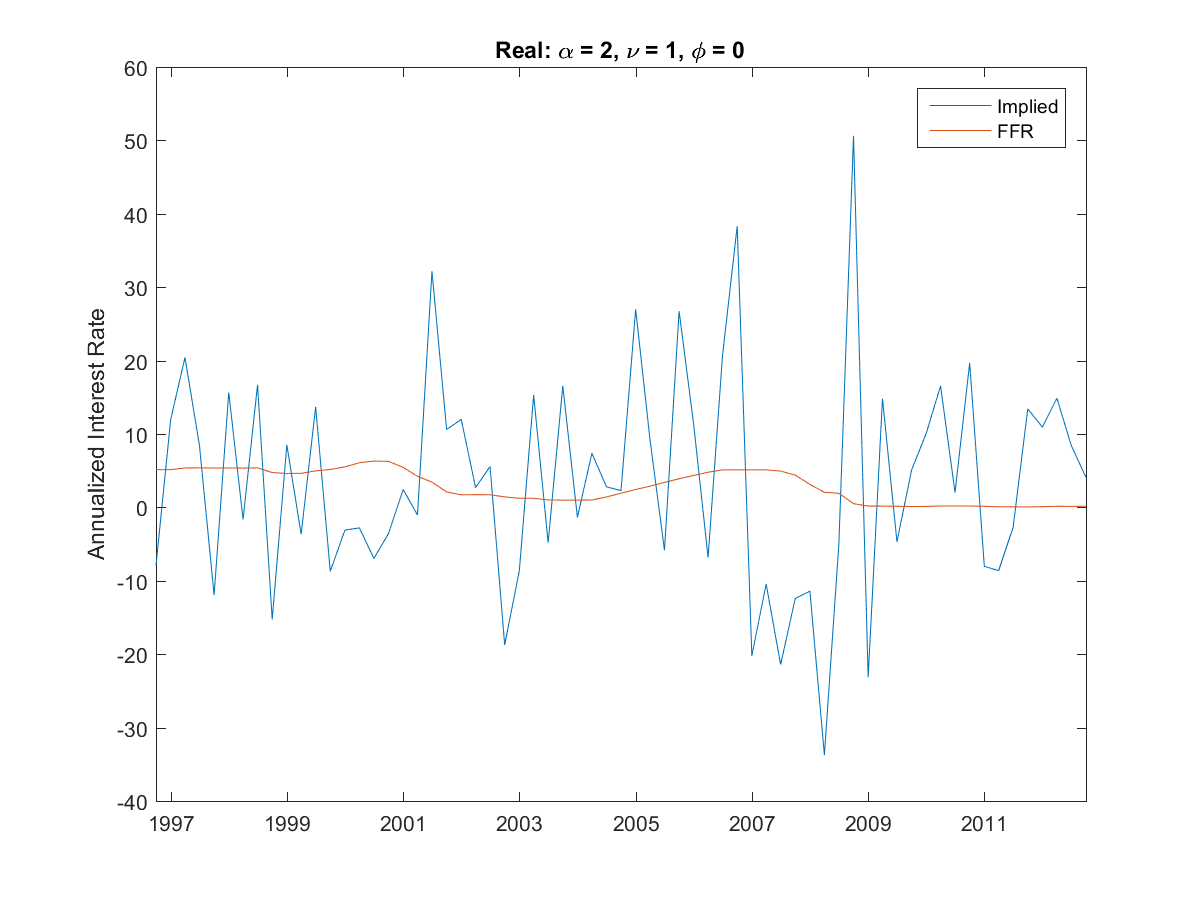
\includegraphics[width=0.4\textwidth]{figs/implied-vs-ffr/cex-nonbondholders/real_alpha2} \\
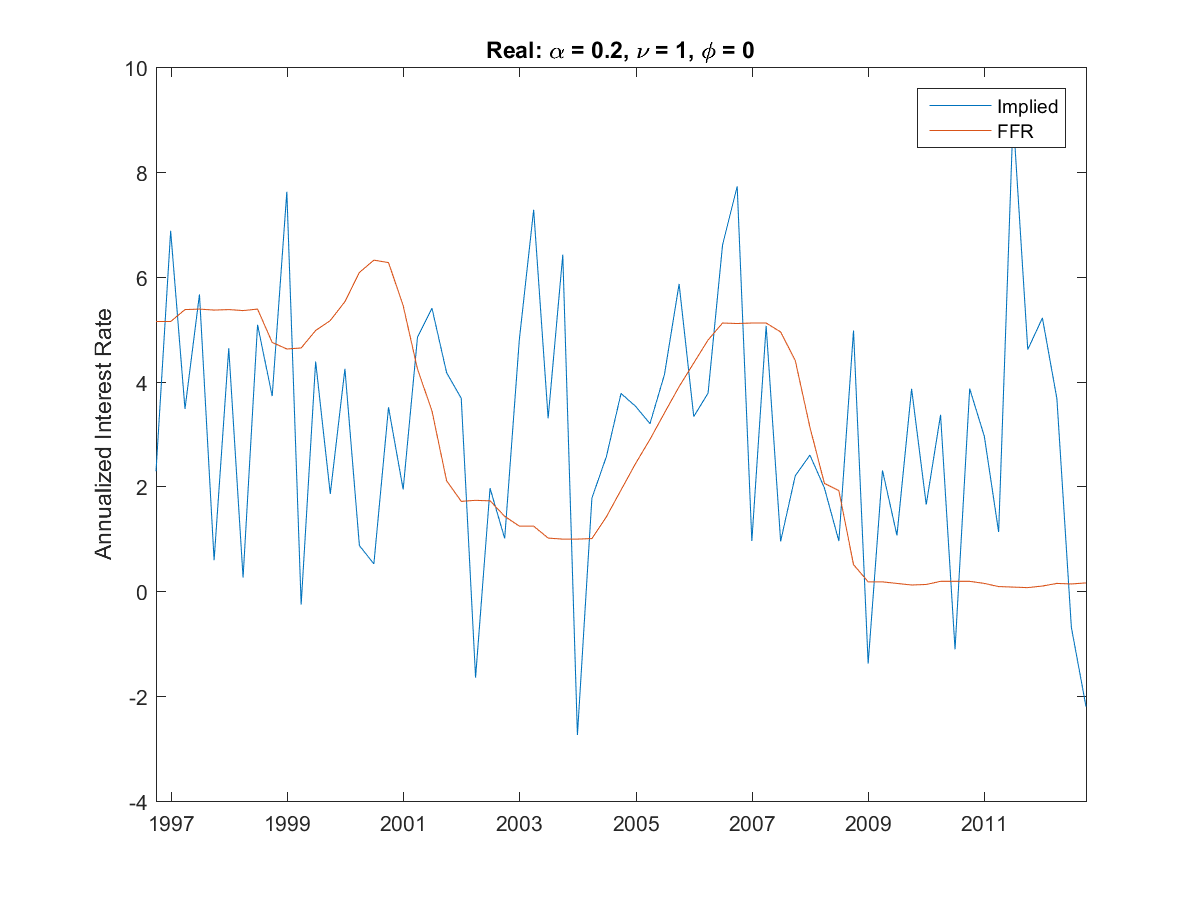
\includegraphics[width=0.4\textwidth]{figs/implied-vs-ffr/cex-bondholders/real_alpha_point2} & 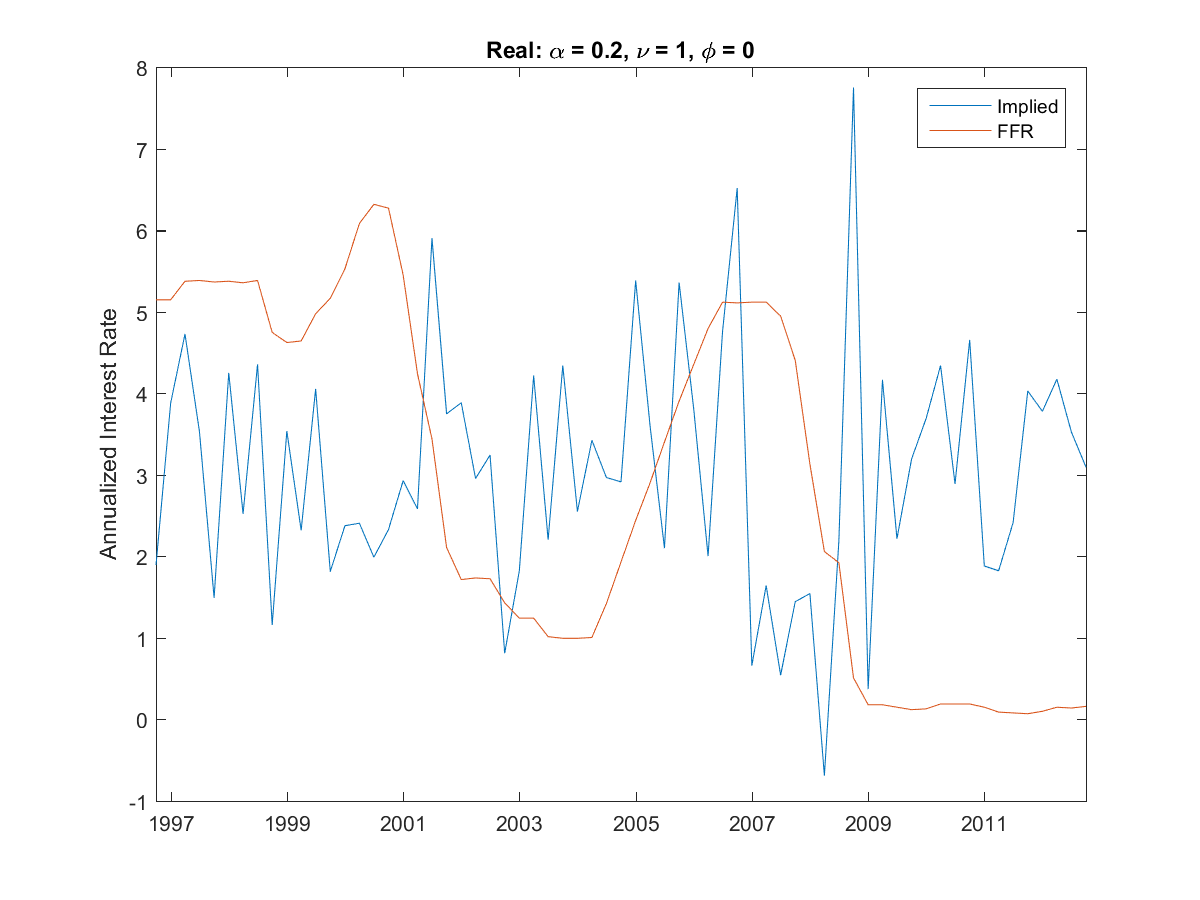
\includegraphics[width=0.4\textwidth]{figs/implied-vs-ffr/cex-nonbondholders/real_alpha_point2}
\end{tabular}
\end{center}
\end{frame}

\begin{frame}{Results: Nominal ($\alpha = 0.2$)}
\begin{center}
\begin{tabular}{lccc}
                   & FFR  & CEX Bond       & CEX Nonbond \\ \hline
Mean               & 2.83 & 5.52           & 5.49 \\
SD                 & 2.19 & 1.91           & 1.59 \\
Corr(Implied, FFR) & ---  & \textbf{0.193} & \textbf{-0.015} \\
Coef(Spread, FFR)  & ---  & -0.549         & -0.647 \\
                   &      & (0.199)        & (0.135)
\end{tabular}
\end{center}
\end{frame}

\begin{frame}{Results: Real ($\alpha = 0.2$)}
\begin{center}
\begin{tabular}{lccc}
                   & FFR   & CEX Bond       & CEX Nonbond \\ \hline
Mean               & 0.353 & 3.06           & 3.05 \\
SD                 & 2.58  & 2.50           & 1.50 \\
Corr(Implied, FFR) & ---   & \textbf{0.235} & \textbf{0.268} \\
Coef(Spread, FFR)  & ---   & -0.527         & -0.650 \\
                   &       & (0.204)        & (0.149) \\
\end{tabular}
\end{center}
\end{frame}

\begin{frame}{Conclusions}
\begin{itemize}
\item Clear difference between bondholders and nonbonders in correlations of nominal rates; no difference for real rates
\item Aggregating household-level consumption at quarter level still very noisy
\item Small sample size even with most generous definition of bondholders
\item EIS ($= \frac{1}{\alpha}$) of 5 not out of the realm of possibility in estimates in literature
\item Negative correlation of spread and FFR seems unavoidable
\item Results not very conclusive
\end{itemize}
\end{frame}

\begin{frame}{References}
\bibliographystyle{../refs/econ}
\bibliography{../refs/thesis}
\end{frame}



\end{document}